\documentclass[12pt, a4paper]{article}

%----------------------------------------------------------------------------------------
%	PACKAGES
%----------------------------------------------------------------------------------------
\usepackage[utf8]{inputenc}
\usepackage[T1]{fontenc}
\usepackage[french]{babel}
\usepackage{geometry}
\usepackage{graphicx}
\usepackage{amsmath, amssymb, amsfonts}
\usepackage{hyperref}
\usepackage{booktabs}
\usepackage{listings}
\usepackage{xcolor}
\usepackage{float}
\usepackage{titlesec}
\usepackage{caption}
\usepackage{fancyhdr}
\usepackage{enumitem}
\usepackage{colortbl}
\usepackage{tcolorbox}
\usepackage{setspace}
\usepackage{parskip}
\usepackage{needspace}

\tcbuselibrary{skins, breakable}

%----------------------------------------------------------------------------------------
%	COLOR PALETTE
%----------------------------------------------------------------------------------------
\definecolor{accent}{HTML}{1A73E8}       % Google Blue - main accent
\definecolor{accentdark}{HTML}{0D47A1}   % Darker blue for headings
\definecolor{accentlight}{HTML}{E8F0FE}  % Very light blue for table rows
\definecolor{textmain}{HTML}{212121}      % Near-black for body text
\definecolor{textsecond}{HTML}{5F6368}    % Gray for secondary text
\definecolor{rulecolor}{HTML}{DADCE0}     % Light gray for rules

% Code listing colors (dark theme)
\definecolor{codebg}{HTML}{1E1E2E}
\definecolor{codefg}{HTML}{CDD6F4}
\definecolor{codekw}{HTML}{89B4FA}
\definecolor{codestr}{HTML}{FAB387}
\definecolor{codecom}{HTML}{6C7086}
\definecolor{codenum}{HTML}{45475A}
\definecolor{codeborder}{HTML}{313244}

%----------------------------------------------------------------------------------------
%	PAGE LAYOUT
%----------------------------------------------------------------------------------------
\geometry{
    top=2.5cm,
    bottom=2.5cm,
    left=2.5cm,
    right=2.5cm
}

\graphicspath{{pictures/}}

\setstretch{1.15}

%----------------------------------------------------------------------------------------
%	HYPERLINKS
%----------------------------------------------------------------------------------------
\hypersetup{
    colorlinks=true,
    linkcolor=accentdark,
    filecolor=accent,      
    urlcolor=accent,
    citecolor=accentdark
}

%----------------------------------------------------------------------------------------
%	HEADERS & FOOTERS
%----------------------------------------------------------------------------------------
\pagestyle{fancy}
\fancyhf{}
\fancyhead[L]{\small\color{textsecond}\textit{STREAMSIGHT}}
\fancyhead[R]{\small\color{textsecond}\textit{D\'etection d'anomalies en temps r\'eel}}
\fancyfoot[C]{\small\color{textsecond}\thepage}
\renewcommand{\headrulewidth}{0.4pt}
\renewcommand{\headrule}{\hbox to\headwidth{\color{rulecolor}\leaders\hrule height \headrulewidth\hfill}}
\renewcommand{\footrulewidth}{0pt}

%----------------------------------------------------------------------------------------
%	SECTION STYLING
%----------------------------------------------------------------------------------------
\titleformat{\section}
    {\needspace{6\baselineskip}\Large\bfseries\color{accentdark}}
    {\thesection.}{0.5em}{}
    [\vspace{2pt}{\color{accent}\titlerule[1pt]}]

\titleformat{\subsection}
    {\needspace{4\baselineskip}\large\bfseries\color{textmain}}
    {\thesubsection}{0.5em}{}

\titlespacing*{\section}{0pt}{18pt}{8pt}
\titlespacing*{\subsection}{0pt}{12pt}{6pt}

% Prevent widows and orphans (lone lines at top/bottom of page)
\widowpenalty=10000
\clubpenalty=10000
\raggedbottom

%----------------------------------------------------------------------------------------
%	TABLE STYLING
%----------------------------------------------------------------------------------------
\newcommand{\tablemark}[1]{\textbf{\color{accentdark}#1}}

%----------------------------------------------------------------------------------------
%	CODE LISTING STYLE
%----------------------------------------------------------------------------------------
\lstdefinestyle{mystyle}{
    backgroundcolor=\color{codebg},   
    commentstyle=\color{codecom}\itshape,
    keywordstyle=\color{codekw}\bfseries,
    numberstyle=\tiny\color{codenum},
    stringstyle=\color{codestr},
    basicstyle=\ttfamily\small\color{codefg},
    breakatwhitespace=false,         
    breaklines=true,                 
    captionpos=b,                    
    keepspaces=true,                 
    numbers=left,                    
    numbersep=8pt,                  
    showspaces=false,                
    showstringspaces=false,
    showtabs=false,                  
    tabsize=2,
    frame=single,
    rulecolor=\color{codeborder},
    xleftmargin=12pt,
    framexleftmargin=8pt,
    aboveskip=12pt,
    belowskip=8pt
}
\lstset{style=mystyle}

%----------------------------------------------------------------------------------------
%	CAPTION STYLING
%----------------------------------------------------------------------------------------
\captionsetup{
    font={small},
    labelfont={bf, color=accentdark},
    textfont={color=textsecond},
    skip=8pt
}

%----------------------------------------------------------------------------------------
%	CUSTOM BOXES
%----------------------------------------------------------------------------------------
\newtcolorbox{infobox}[1][]{
    colback=accentlight,
    colframe=accent,
    coltitle=white,
    fonttitle=\bfseries,
    boxrule=0pt,
    leftrule=3pt,
    arc=0pt,
    outer arc=0pt,
    left=10pt,
    right=10pt,
    top=8pt,
    bottom=8pt,
    #1
}

%----------------------------------------------------------------------------------------
%	LIST STYLING
%----------------------------------------------------------------------------------------
\setlist[itemize]{
    itemsep=4pt,
    parsep=2pt,
    label={\color{accent}\textbullet}
}
\setlist[enumerate]{
    itemsep=4pt,
    parsep=2pt,
    label={\color{accent}\textbf{\arabic*.}}
}

%----------------------------------------------------------------------------------------
%	DOCUMENT START
%----------------------------------------------------------------------------------------
\begin{document}
\color{textmain}

%----------------------------------------------------------------------------------------
%	PAGE DE TITRE
%----------------------------------------------------------------------------------------
\begin{titlepage}
    \thispagestyle{empty}
    \begin{center}
        
        \vspace*{1.5cm}
        
        % Top accent line
        {\color{accent}\rule{\textwidth}{2pt}}
        
        \vspace{1.2cm}
        
        {\fontsize{36}{42}\selectfont\bfseries\color{accentdark} STREAMSIGHT}
        
        \vspace{0.6cm}
        
        {\Large\color{textsecond} Plateforme de d\'etection d'anomalies\\[4pt] en temps r\'eel sur le march\'e des cryptomonnaies}
        
        \vspace{0.5cm}
        
        {\color{accent}\rule{0.4\textwidth}{1pt}}
        
        \vspace{2.5cm}
        
        {\large\color{textmain}
        \textbf{Auteurs}\\[10pt]
        Farouk BENKHLIFA\\[4pt]
        Mohammed Anes BOUCETLA
        }
        
        \vfill
        
        {\color{textsecond}
        \textbf{ENSTTIC}\\[8pt]
        Rapport soumis pour le module :\\[4pt]
        \textit{Big Data \& Streaming en Temps R\'eel}
        }
        
        \vspace{1.2cm}
        
        {\color{accent}\rule{\textwidth}{2pt}}
        
        \vspace{0.6cm}
        
        {\Large\color{textsecond} F\'evrier 2026}
        
    \end{center}
\end{titlepage}

%----------------------------------------------------------------------------------------
%	R\'ESUM\'E
%----------------------------------------------------------------------------------------
\thispagestyle{plain}

\begin{infobox}[title=R\'esum\'e]
    \noindent 
    Dans le domaine hautement volatile du trading de cryptomonnaies, les m\'ethodes traditionnelles de traitement par lots (batch) ne parviennent pas \`a fournir les informations \`a faible latence n\'ecessaires \`a une gestion efficace des risques. Ce rapport pr\'esente \textbf{STREAMSIGHT}, un pipeline complet d'ing\'enierie de donn\'ees en temps r\'eel con\c{c}u pour d\'etecter les anomalies de march\'e d\`es leur apparition. Le syst\`eme ingère les donn\'ees de transactions BTC/USDT en direct depuis la bourse Binance via WebSocket, met en tampon le flux \`a haut d\'ebit \`a l'aide d'Apache Kafka, et traite les donn\'ees en quasi temps r\'eel avec Apache Spark Structured Streaming.
    
    \vspace{6pt}
    Le moteur analytique principal calcule le prix moyen pond\'er\'e par le volume (VWAP) et les Z-Scores statistiques au sein de fen\^etres temporelles fixes (tumbling windows) pour identifier les mouvements de prix anormaux. Les r\'esultats trait\'es sont stock\'es dans Elasticsearch avec une s\'emantique exactly-once et visualis\'es \`a travers des tableaux de bord interactifs Kibana. L'ensemble de l'infrastructure est conteneuris\'ee avec Docker, d\'emontrant une architecture robuste et \'evolutive adapt\'ee \`a l'ing\'enierie de donn\'ees financi\`eres moderne.
\end{infobox}

\newpage
\tableofcontents
\newpage

%----------------------------------------------------------------------------------------
%	1. INTRODUCTION
%----------------------------------------------------------------------------------------
\section{Introduction}

\subsection{Contexte et probl\'ematique}
Les march\'es de cryptomonnaies fonctionnent en continu, 24 heures sur 24, g\'en\'erant des volumes massifs de donn\'ees de transactions. La nature d\'ecentralis\'ee de ces march\'es entra\^ine une volatilit\'e extr\^eme, o\`u les prix peuvent fluctuer de mani\`ere spectaculaire en quelques secondes. Les approches traditionnelles de traitement par lots, qui traitent les donn\'ees en blocs accumul\'es \`a intervalles r\'eguliers (par exemple, quotidiennement ou toutes les heures), introduisent une latence inacceptable. Le temps qu'une anomalie soit d\'etect\'ee dans un syst\`eme batch, l'opportunit\'e de march\'e ou l'\'ev\'enement de risque est souvent d\'ej\`a pass\'e.

\subsection{Importance du traitement en temps r\'eel}
Sur les march\'es financiers, la latence \'equivaut \`a de l'argent. Les traders algorithmiques et les gestionnaires de risques n\'ecessitent une visibilit\'e en temps r\'eel ou quasi r\'eel sur les conditions du march\'e pour prendre des d\'ecisions \'eclair\'ees. Les architectures de streaming permettent le calcul continu d'indicateurs financiers, rendant possible la d\'etection imm\'ediate de \og flash crashes \fg{} ou de sch\'emas de type \og pump-and-dump \fg{}.

\subsection{Objectifs du projet}
L'objectif principal de STREAMSIGHT est de concevoir et impl\'ementer un pipeline de donn\'ees en temps r\'eel de bout en bout, d\'emontrant les pratiques modernes d'ing\'enierie de donn\'ees. Plus pr\'ecis\'ement, le projet vise \`a :
\begin{itemize}
    \item Ing\'erer des donn\'ees de transactions en direct depuis une bourse publique (Binance).
    \item Assurer la durabilit\'e des donn\'ees et le d\'ecouplage \`a l'aide d'un courtier de messages distribu\'e.
    \item Effectuer un traitement de flux avec \'etat (stateful) pour calculer des m\'etriques complexes (VWAP).
    \item D\'etecter les anomalies statistiques en utilisant les Z-Scores \`a la vol\'ee.
    \item Visualiser les r\'esultats dans un tableau de bord convivial.
\end{itemize}

%----------------------------------------------------------------------------------------
%	2. ARCHITECTURE DU SYST\`EME
%----------------------------------------------------------------------------------------
\section{Architecture du syst\`eme}

STREAMSIGHT suit une architecture de streaming lin\'eaire de style Lambda compos\'ee de cinq \'etapes distinctes.

\subsection{\'Etapes du pipeline}
\begin{enumerate}
    \item \textbf{Ingestion :} Un script producteur en Python se connecte \`a l'API WebSocket de Binance pour recevoir les \'ev\'enements de transactions bruts de la paire BTC/USDT.
    \item \textbf{Mise en tampon :} Les \'ev\'enements bruts sont s\'erialis\'es en JSON et publi\'es dans le topic \texttt{crypto\_trades} d'Apache Kafka. Kafka agit comme amortisseur, d\'ecouplant la couche d'ingestion de la couche de traitement.
    \item \textbf{Traitement :} Apache Spark Structured Streaming consomme le topic Kafka. Il analyse le JSON, g\`ere les donn\'ees tardives via le watermarking, et agr\`ege les transactions dans des fen\^etres temporelles fixes de 10 secondes pour calculer les m\'etriques financi\`eres.
    \item \textbf{Stockage :} Les r\'esultats agr\'eg\'es, y compris les indicateurs d'anomalies, sont \'ecrits dans un index Elasticsearch nomm\'e \texttt{streamsight-trades}.
    \item \textbf{Visualisation :} Kibana se connecte \`a Elasticsearch pour afficher des tableaux de bord en temps r\'eel, permettant aux utilisateurs de surveiller les tendances de prix et les alertes d'anomalies.
\end{enumerate}

\subsection{Diagramme de flux de donn\'ees}
Le diagramme suivant illustre le flux unidirectionnel des donn\'ees \`a travers le syst\`eme :

\begin{lstlisting}[language=bash, caption=Flux de donn\'ees de bout en bout de STREAMSIGHT]
+-------------+      +------------------+      +--------------+
|   Binance   |      |  Python Producer |      | Apache Kafka |
|  WebSocket  | ---> |    (Ingestion)   | ---> |   (Tampon)   |
+-------------+      +------------------+      +--------------+
                                                      |
                                                      v
+-------------+      +------------------+      +--------------+
|    Kibana   |      |   Elasticsearch  |      | Apache Spark |
| (Dashboard) | <--- |    (Stockage)    | <--- | (Traitement) |
+-------------+      +------------------+      +--------------+
\end{lstlisting}

\subsection{Infrastructure}
L'infrastructure est orchestr\'ee \`a l'aide de Docker Compose, qui g\`ere quatre conteneurs principaux : Zookeeper (coordinateur Kafka), Kafka (courtier de messages), Elasticsearch (stockage) et Kibana (visualisation sur le port 5601).

\begin{figure}[htbp]
    \centering
    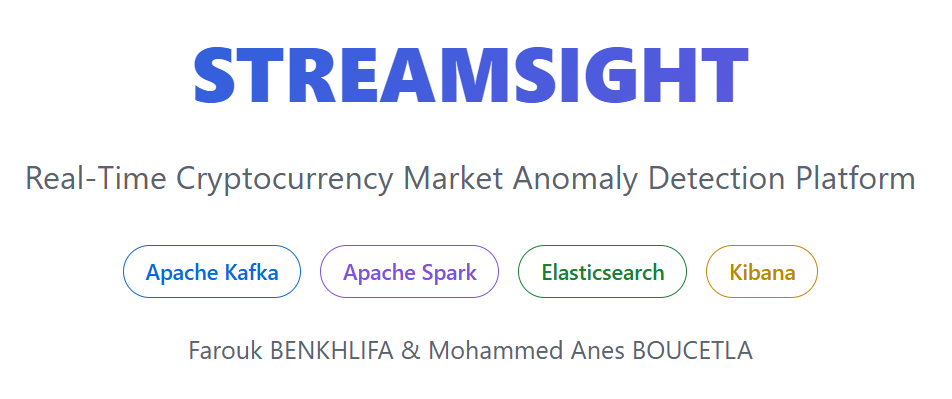
\includegraphics[width=\textwidth]{fig1_docker_compose_up.png}
    \caption{Lancement de l'infrastructure avec \texttt{docker compose up -d}. Les quatre conteneurs (Zookeeper, Kafka, Elasticsearch, Kibana) sont d\'emarr\'es en mode d\'etach\'e.}
    \label{fig:docker_compose_up}
\end{figure}

\begin{figure}[htbp]
    \centering
    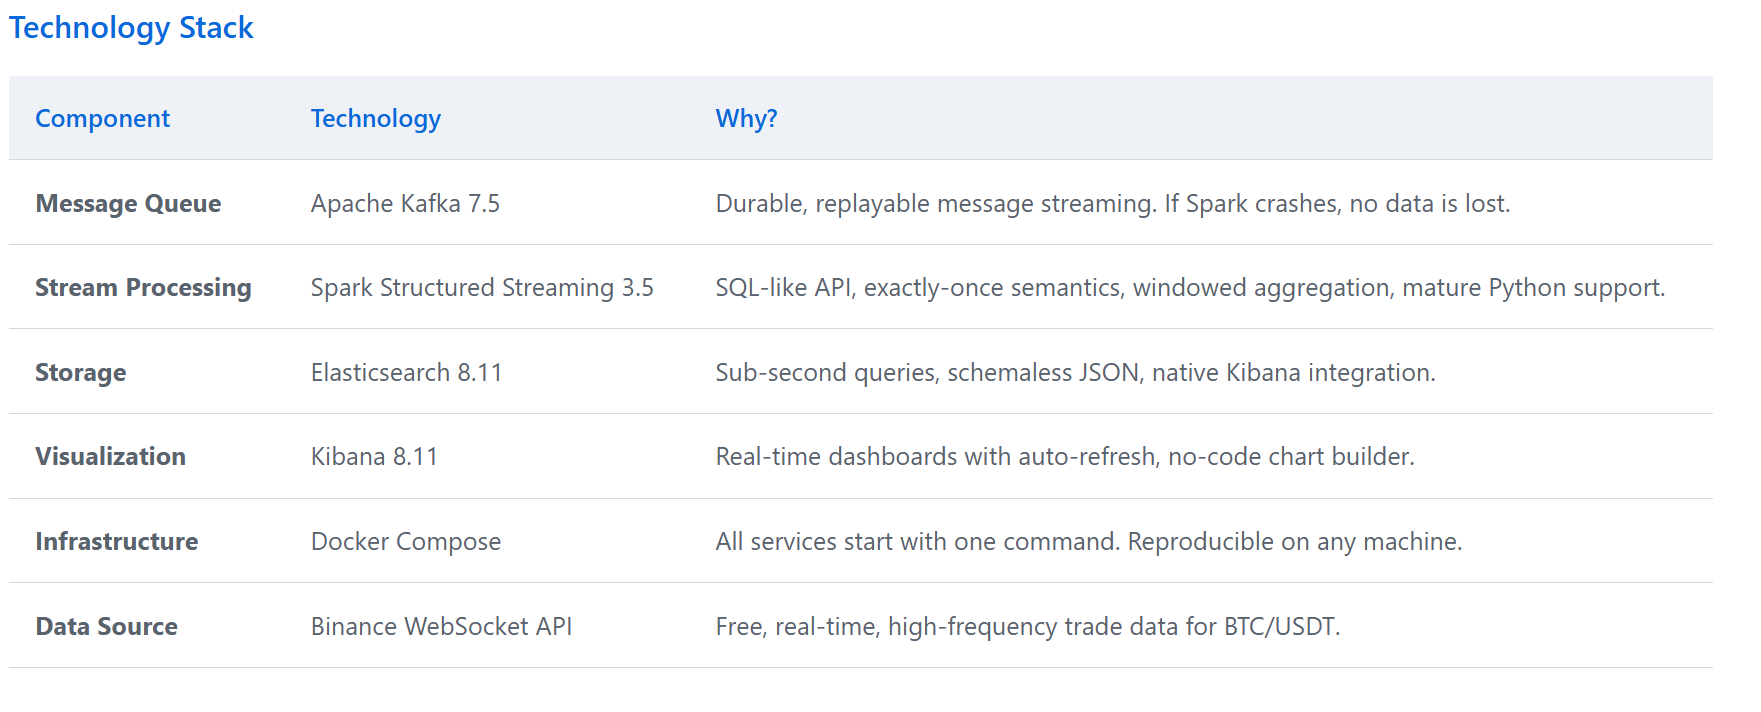
\includegraphics[width=\textwidth]{fig3_docker_running.png}
    \caption{Tous les conteneurs de l'infrastructure dans un \'etat de fonctionnement sain, v\'erifi\'e avec \texttt{docker compose ps}.}
    \label{fig:docker_running}
\end{figure}

%----------------------------------------------------------------------------------------
%	3. PILE TECHNOLOGIQUE
%----------------------------------------------------------------------------------------
\section{Pile technologique}

Le projet utilise une pile de technologies open source choisies pour leur fiabilit\'e et leur large adoption dans l'industrie.

\begin{table}[htbp]
\centering
\caption{R\'esum\'e de la pile technologique}
\rowcolors{2}{accentlight}{white}
\begin{tabular}{llcl}
\toprule
\tablemark{Composant} & \tablemark{Technologie} & \tablemark{Version} & \tablemark{R\^ole} \\
\midrule
Traitement de flux & Apache Spark & 3.5.7 & Agr\'egation fen\^etr\'ee \& d\'etection d'anomalies \\
File de messages & Apache Kafka & 7.5.0 & Mise en tampon fiable des messages \\
Coordination & Apache Zookeeper & 7.5.0 & Coordinateur du cluster Kafka \\
Base de donn\'ees & Elasticsearch & 8.11.4 & Stockage et analytique de s\'eries temporelles \\
Visualisation & Kibana & 8.11.4 & Tableaux de bord en direct \\
Conteneurisation & Docker Compose & Derni\`ere & Orchestration de l'infrastructure \\
Langage & Python & 3.10 & Logique applicative (PySpark) \\
\bottomrule
\end{tabular}
\end{table}

%----------------------------------------------------------------------------------------
%	4. CHOIX DE CONCEPTION ET COMPARAISONS
%----------------------------------------------------------------------------------------
\section{Choix de conception et comparaisons technologiques}

\subsection{Courtier de messages : Apache Kafka vs. Redis Pub/Sub}
Apache Kafka a \'et\'e s\'electionn\'e plut\^ot que Redis Pub/Sub principalement en raison de sa durabilit\'e et de ses capacit\'es de rejeu, qui sont essentielles pour les pipelines de donn\'ees financi\`eres o\`u la perte de donn\'ees est inacceptable.

\begin{table}[htbp]
\centering
\caption{Kafka vs. Redis Pub/Sub}
\rowcolors{2}{accentlight}{white}
\begin{tabular}{lll}
\toprule
\tablemark{Crit\`ere} & \tablemark{Apache Kafka} & \tablemark{Redis Pub/Sub} \\
\midrule
Persistance des messages & Persist\'e sur disque (durable) & Fire-and-forget (volatile) \\
Rejeu consommateur & Support\'e (recherche par offset) & Non support\'e \\
Contre-pression & Le consommateur tire les donn\'ees & Le producteur peut surcharger \\
D\'ebit & Extr\^emement \'elev\'e & \'Elev\'e \\
Complexit\'e & \'Elev\'ee (n\'ecessite Zookeeper) & Faible \\
\bottomrule
\end{tabular}
\end{table}

\subsection{Processeur de flux : Spark Structured Streaming vs. Apache Flink}
Bien que Flink offre une latence native plus faible, Spark a \'et\'e choisi pour son API Python (PySpark) mature et sa syntaxe de type SQL, qui ont simplifi\'e l'impl\'ementation des agr\'egations fen\^etr\'ees.

\begin{table}[htbp]
\centering
\caption{Spark Structured Streaming vs. Apache Flink}
\rowcolors{2}{accentlight}{white}
\begin{tabular}{lll}
\toprule
\tablemark{Crit\`ere} & \tablemark{Spark Streaming} & \tablemark{Apache Flink} \\
\midrule
Latence & Micro-batch (secondes) & \'Ev\'enementiel (sub-seconde) \\
Exactly-Once & Support\'e (Checkpoints) & Support\'e (Checkpoints) \\
API Python & Mature (PySpark) & En am\'elioration (PyFlink) \\
Courbe d'apprentissage & Mod\'er\'ee (type SQL) & Abrupte \\
\'Ecosyst\`eme & Massif (MLlib, SQL) & Centr\'e sur le streaming \\
\bottomrule
\end{tabular}
\end{table}

\subsection{Stockage : Elasticsearch vs. TimescaleDB}
Elasticsearch a \'et\'e s\'electionn\'e pour son int\'egration native avec Kibana, permettant un prototypage rapide de tableaux de bord sans n\'ecessiter un outil de visualisation s\'epar\'e comme Grafana.

\begin{table}[htbp]
\centering
\caption{Elasticsearch vs. TimescaleDB}
\rowcolors{2}{accentlight}{white}
\begin{tabular}{lll}
\toprule
\tablemark{Crit\`ere} & \tablemark{Elasticsearch} & \tablemark{TimescaleDB} \\
\midrule
Vitesse de requ\^ete & Rapide pour recherche/agr\'eg. & Rapide pour s\'eries temporelles \\
Flexibilit\'e du sch\'ema & Sans sch\'ema (JSON) & Strict (SQL) \\
Int\'egration Kibana & Native & N\'ecessite Grafana \\
Transactions ACID & Coh\'erence \'eventuelle & ACID complet \\
Agr\'egation & Agr\'egations par buckets puissantes & SQL standard \\
\bottomrule
\end{tabular}
\end{table}

%----------------------------------------------------------------------------------------
%	5. IMPL\'EMENTATION
%----------------------------------------------------------------------------------------
\section{Impl\'ementation}

\subsection{Ingestion des donn\'ees}
Le script d'ingestion, \texttt{binance\_to\_kafka.py}, \'etablit une connexion WebSocket persistante vers l'endpoint de l'API Binance :
\texttt{wss://stream.binance.com:9443/ws/btcusdt@trade}.

\`A la r\'eception d'un message de transaction, le script extrait le symbole, le prix, la quantit\'e et l'horodatage de l'\'ev\'enement (en millisecondes Unix). Les donn\'ees sont s\'erialis\'ees en JSON et publi\'ees dans le topic Kafka.

\begin{lstlisting}[language=Python, caption=Construction JSON du producteur Python]
# Dans le callback WebSocket
record = {
    "symbol": trade["s"],          # Paire de trading (ex: BTCUSDT)
    "price": float(trade["p"]),    # Prix de la transaction
    "quantity": float(trade["q"]), # Volume de la transaction
    "event_time": trade["T"]       # Horodatage (ms)
}

# Publication vers Kafka
producer.send(KAFKA_TOPIC, value=record)
\end{lstlisting}

\begin{figure}[htbp]
    \centering
    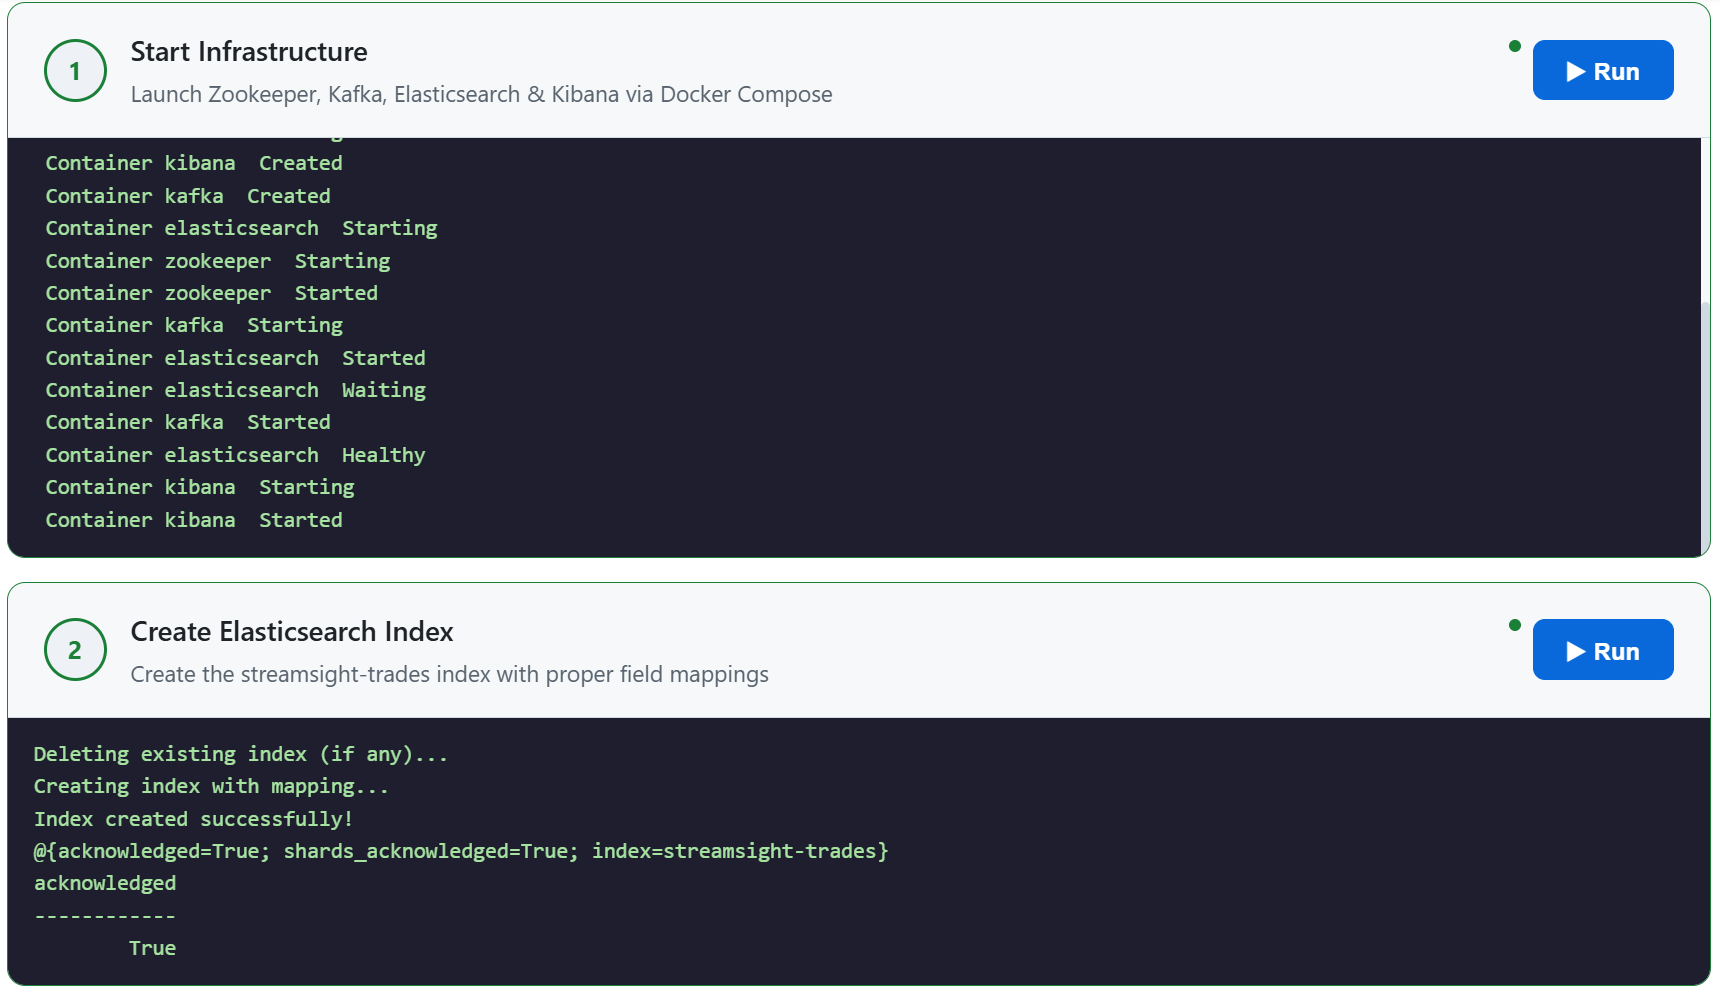
\includegraphics[width=\textwidth]{fig9_producer_output.png}
    \caption{Le script producteur Binance en cours d'ex\'ecution dans le terminal. Chaque ligne repr\'esente une transaction BTC/USDT en direct re\c{c}ue depuis le WebSocket et transmise au topic Kafka \texttt{crypto\_trades}.}
    \label{fig:producer_output}
\end{figure}

\subsection{Configuration du traitement de flux}
La logique principale r\'eside dans \texttt{spark\_streaming.py}. La session Spark est configur\'ee pour fonctionner localement en utilisant le master \texttt{local[*]}. Elle lit depuis Kafka \`a partir des offsets \texttt{latest} pour ne traiter que les donn\'ees en direct.

De mani\`ere cruciale, un watermark de \textbf{5 secondes} est appliqu\'e sur le champ \texttt{event\_time}. Cela indique \`a Spark de maintenir l'\'etat pour les donn\'ees arrivant avec un retard allant jusqu'\`a 5 secondes, apr\`es quoi l'\'etat interm\'ediaire est supprim\'e pour g\'erer l'utilisation de la m\'emoire. Les donn\'ees sont regroup\'ees dans des \textbf{fen\^etres temporelles fixes de 10 secondes}.

\begin{figure}[htbp]
    \centering
    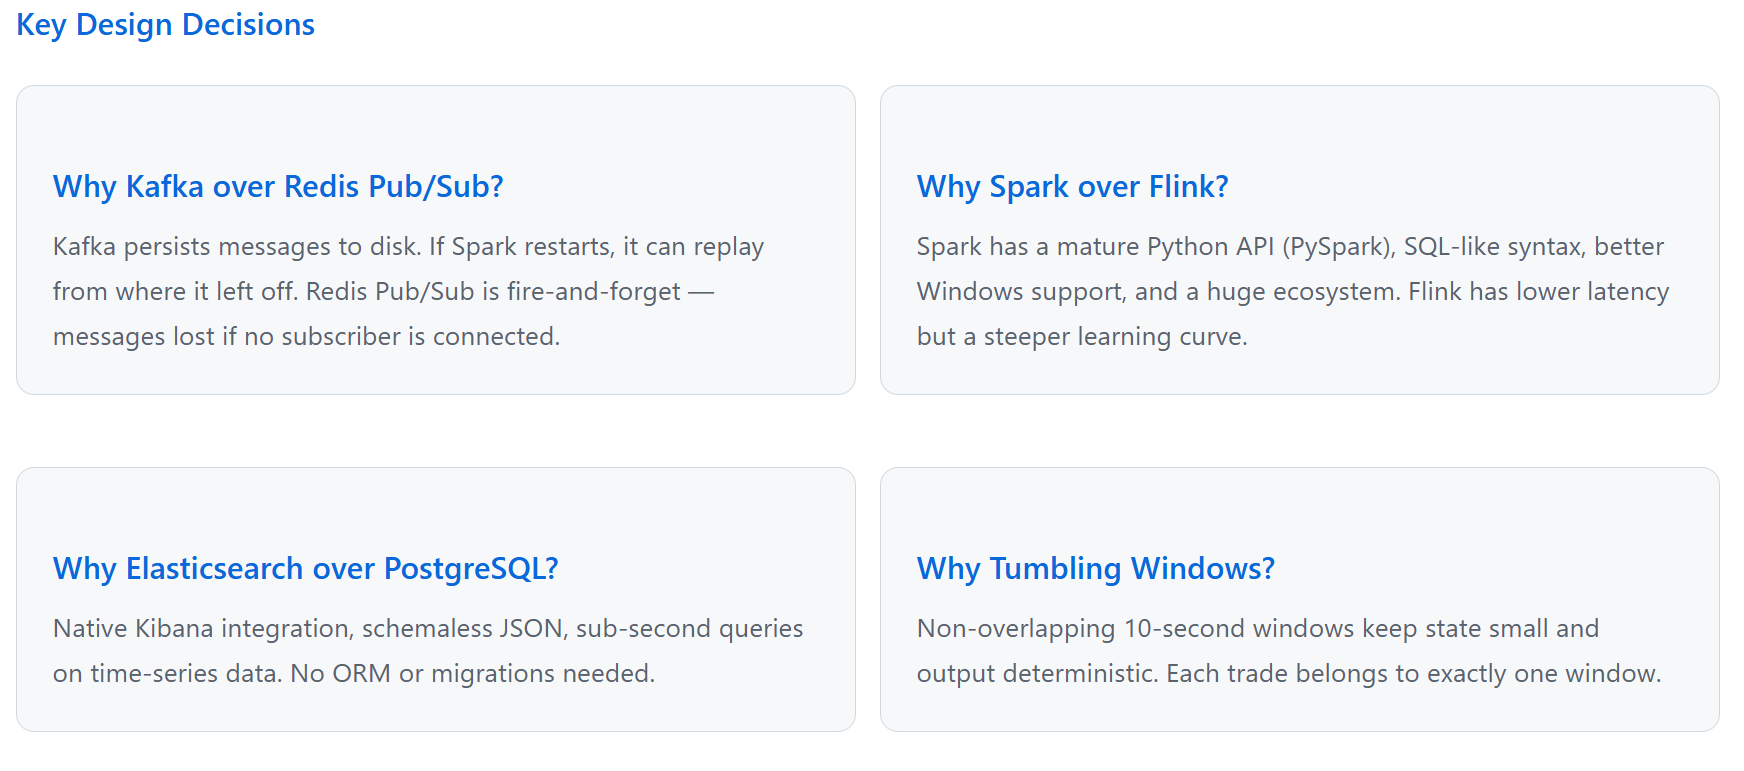
\includegraphics[width=\textwidth]{fig5_spark_submit.png}
    \caption{Lancement du job Spark Structured Streaming via \texttt{spark-submit} avec les packages de connecteurs Kafka et Elasticsearch.}
    \label{fig:spark_submit}
\end{figure}

\begin{figure}[htbp]
    \centering
    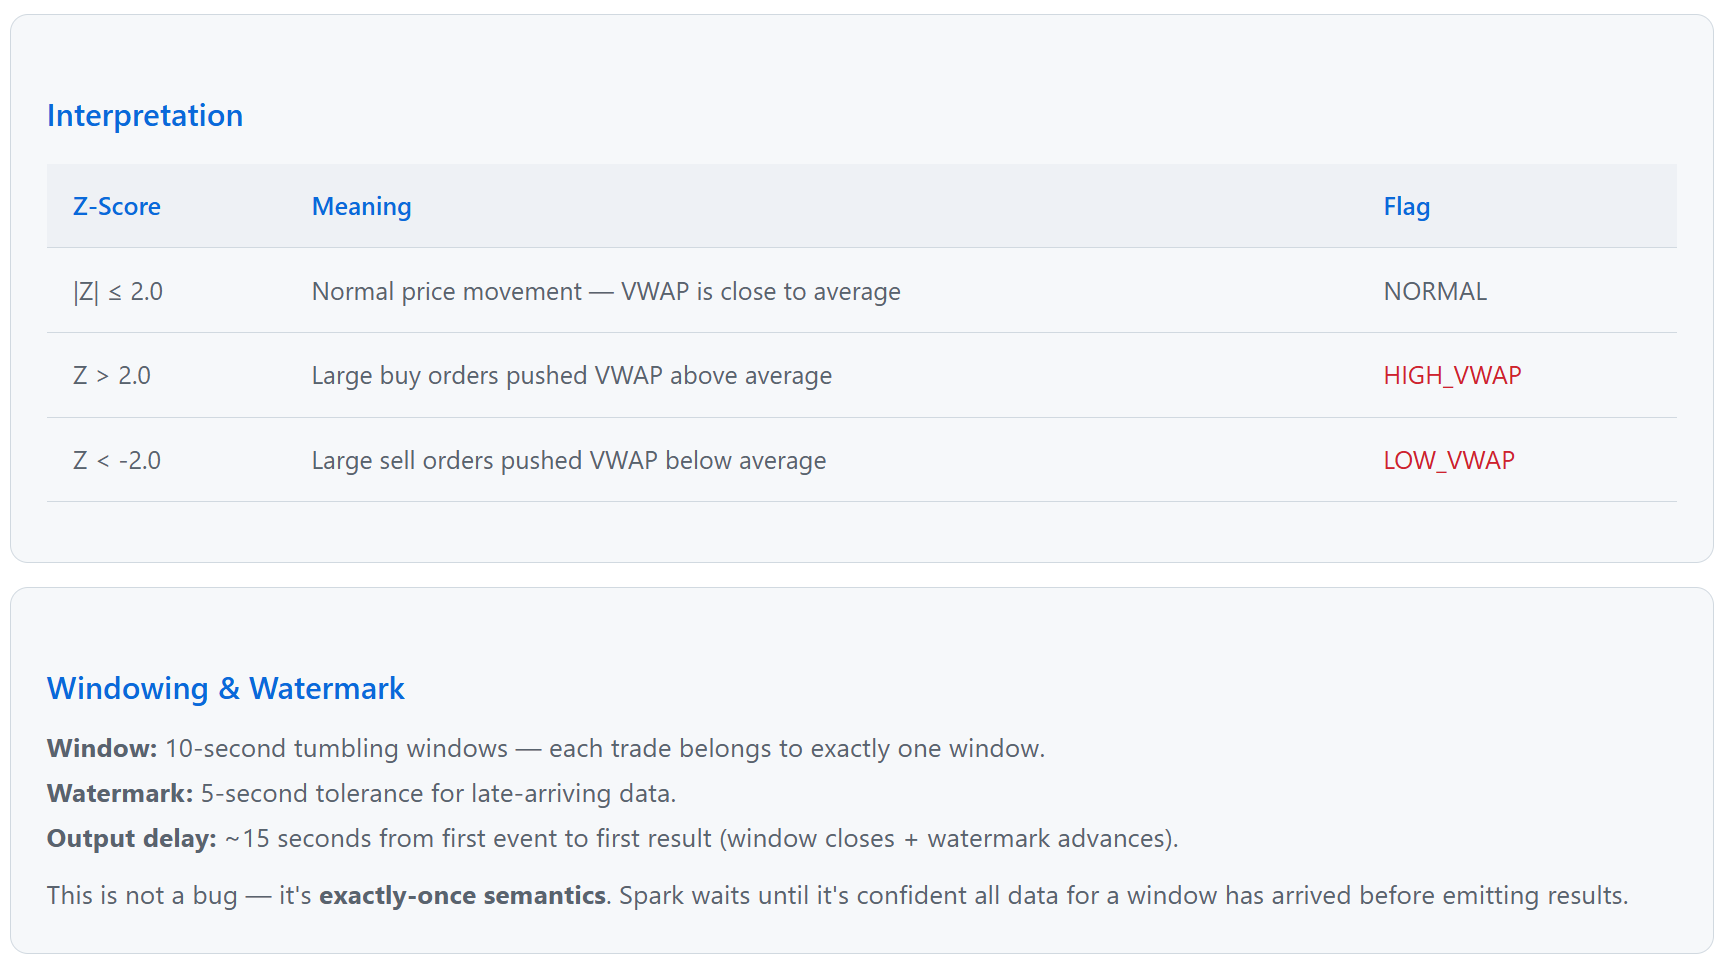
\includegraphics[width=\textwidth]{fig7_spark_output.png}
    \caption{Sortie console de Spark Structured Streaming. Chaque ligne repr\'esente une fen\^etre temporelle de 10 secondes, affichant le VWAP calcul\'e, le Z-score, le nombre de transactions et la classification d'anomalie.}
    \label{fig:spark_output}
\end{figure}

\subsection{Calcul du VWAP}
Le \textbf{prix moyen pond\'er\'e par le volume} (VWAP -- Volume-Weighted Average Price) est un indicateur de r\'ef\'erence en trading qui donne le prix moyen auquel un titre a \'et\'e n\'egoci\'e tout au long de la journ\'ee, en tenant compte \`a la fois du volume et du prix. Il est calcul\'e comme suit :

\begin{tcolorbox}[
    colback=accentlight,
    colframe=accent,
    boxrule=0.5pt,
    arc=4pt,
    left=12pt, right=12pt, top=10pt, bottom=10pt
]
\begin{equation}
    VWAP = \frac{\displaystyle\sum_{i=1}^{n} (P_i \times Q_i)}{\displaystyle\sum_{i=1}^{n} Q_i}
\end{equation}
\end{tcolorbox}

\noindent O\`u :
\begin{itemize}
    \item $P_i$ est le prix de la transaction $i$.
    \item $Q_i$ est la quantit\'e de la transaction $i$.
    \item $n$ est le nombre total de transactions dans la fen\^etre.
\end{itemize}

Le VWAP est pr\'ef\'er\'e \`a une moyenne simple car il emp\^eche les petites transactions insignifiantes de fausser la m\'etrique de prix.

\subsection{D\'etection d'anomalies (Z-Score)}
Pour d\'etecter les anomalies, le syst\`eme calcule le Z-Score du VWAP par rapport au prix moyen simple au sein de la m\^eme fen\^etre :

\begin{tcolorbox}[
    colback=accentlight,
    colframe=accent,
    boxrule=0.5pt,
    arc=4pt,
    left=12pt, right=12pt, top=10pt, bottom=10pt
]
\begin{equation}
    Z = \frac{VWAP - \mu}{\sigma}
\end{equation}
\end{tcolorbox}

\noindent O\`u :
\begin{itemize}
    \item $\mu$ est le prix moyen simple dans la fen\^etre.
    \item $\sigma$ est l'\'ecart-type des prix dans la fen\^etre.
\end{itemize}

Le syst\`eme signale une fen\^etre comme anomalie si $|Z| > 2.0$. Dans une distribution normale, ce seuil couvre environ 95\,\% des points de donn\'ees, ce qui signifie que toute valeur en dehors de cette plage repr\'esente les 2{,}5\,\% sup\'erieurs ou inf\'erieurs des d\'eviations.

\begin{infobox}
\textbf{Classification des anomalies :}
\begin{itemize}[leftmargin=*]
    \item \textbf{HIGH\_VWAP} $(Z > 2.0)$ --- Ordres d'achat importants poussant le VWAP significativement au-dessus de la moyenne.
    \item \textbf{LOW\_VWAP} $(Z < -2.0)$ --- Ordres de vente importants poussant le VWAP significativement en dessous de la moyenne.
    \item \textbf{NORMAL} $(-2.0 \leq Z \leq 2.0)$ --- Prix dans la plage attendue.
\end{itemize}
\end{infobox}

\subsection{Sch\'ema des donn\'ees}
Voici un exemple de la transformation des donn\'ees brutes en sortie trait\'ee.

\begin{lstlisting}[language=json, caption=Entr\'ee Kafka vs. Sortie Elasticsearch]
// Entree (Message Kafka brut)
{ 
  "symbol": "BTCUSDT", 
  "price": 87928.57, 
  "quantity": 0.00053, 
  "event_time": 1766178316409 
}

// Sortie (Document traite dans Elasticsearch)
{
  "symbol": "BTCUSDT",
  "window_start": 1766177700000,
  "window_end": 1766177710000,
  "total_volume": 5.108,
  "trade_count": 1258,
  "avg_price": 88081.96,
  "vwap": 88078.50,
  "price_stddev": 10.41,
  "zscore": -0.332,
  "is_anomaly": false,
  "anomaly_type": "NORMAL",
  "doc_id": "BTCUSDT_20251219215500"
}
\end{lstlisting}

%----------------------------------------------------------------------------------------
%	6. D\'EMONSTRATION DU SYST\`EME
%----------------------------------------------------------------------------------------
\section{D\'emonstration du syst\`eme}

Cette section pr\'esente des captures d'\'ecran du pipeline en fonctionnement complet, de la couche de visualisation Kibana jusqu'aux documents bruts stock\'es dans Elasticsearch.

\begin{figure}[htbp]
    \centering
    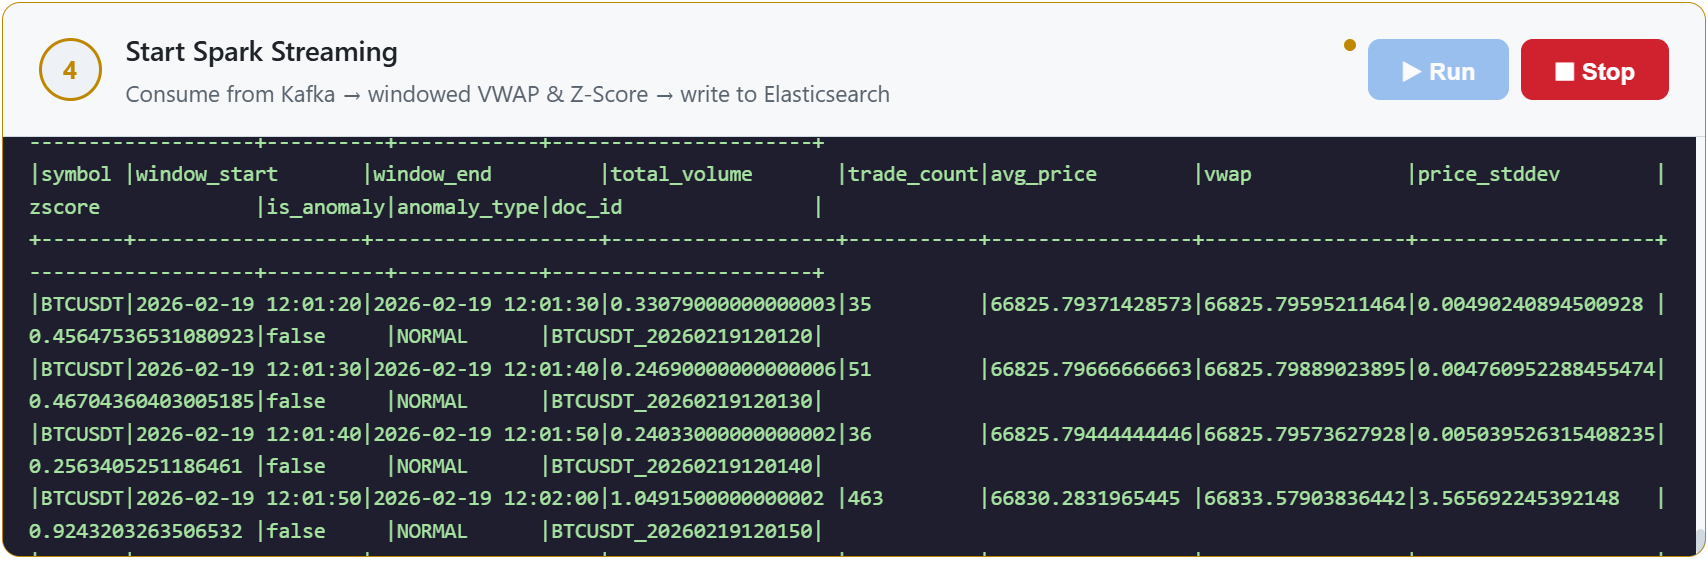
\includegraphics[width=\textwidth]{fig11_kibana_dashboard.png}
    \caption{Tableau de bord principal Kibana montrant l'interface de surveillance en temps r\'eel de STREAMSIGHT. Le tableau de bord affiche les valeurs VWAP BTC/USDT en direct, le volume de transactions par fen\^etre et la s\'erie temporelle du Z-score.}
    \label{fig:kibana_dashboard}
\end{figure}

\begin{figure}[htbp]
    \centering
    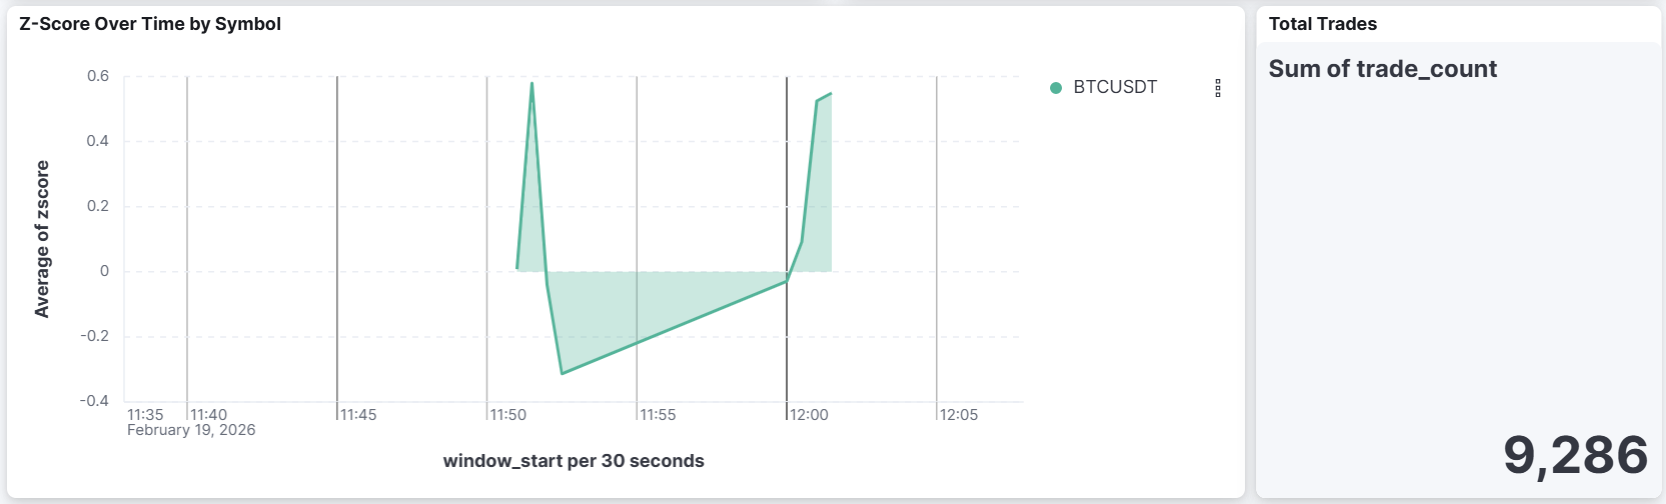
\includegraphics[width=\textwidth]{fig13_kibana_anomaly.png}
    \caption{Panneau de d\'etection d'anomalies Kibana. Les fen\^etres signal\'ees comme \texttt{HIGH\_VWAP} ou \texttt{LOW\_VWAP} (o\`u $|Z| > 2.0$) sont mises en \'evidence, indiquant des d\'eviations de prix statistiquement significatives.}
    \label{fig:kibana_anomaly}
\end{figure}

\begin{figure}[htbp]
    \centering
    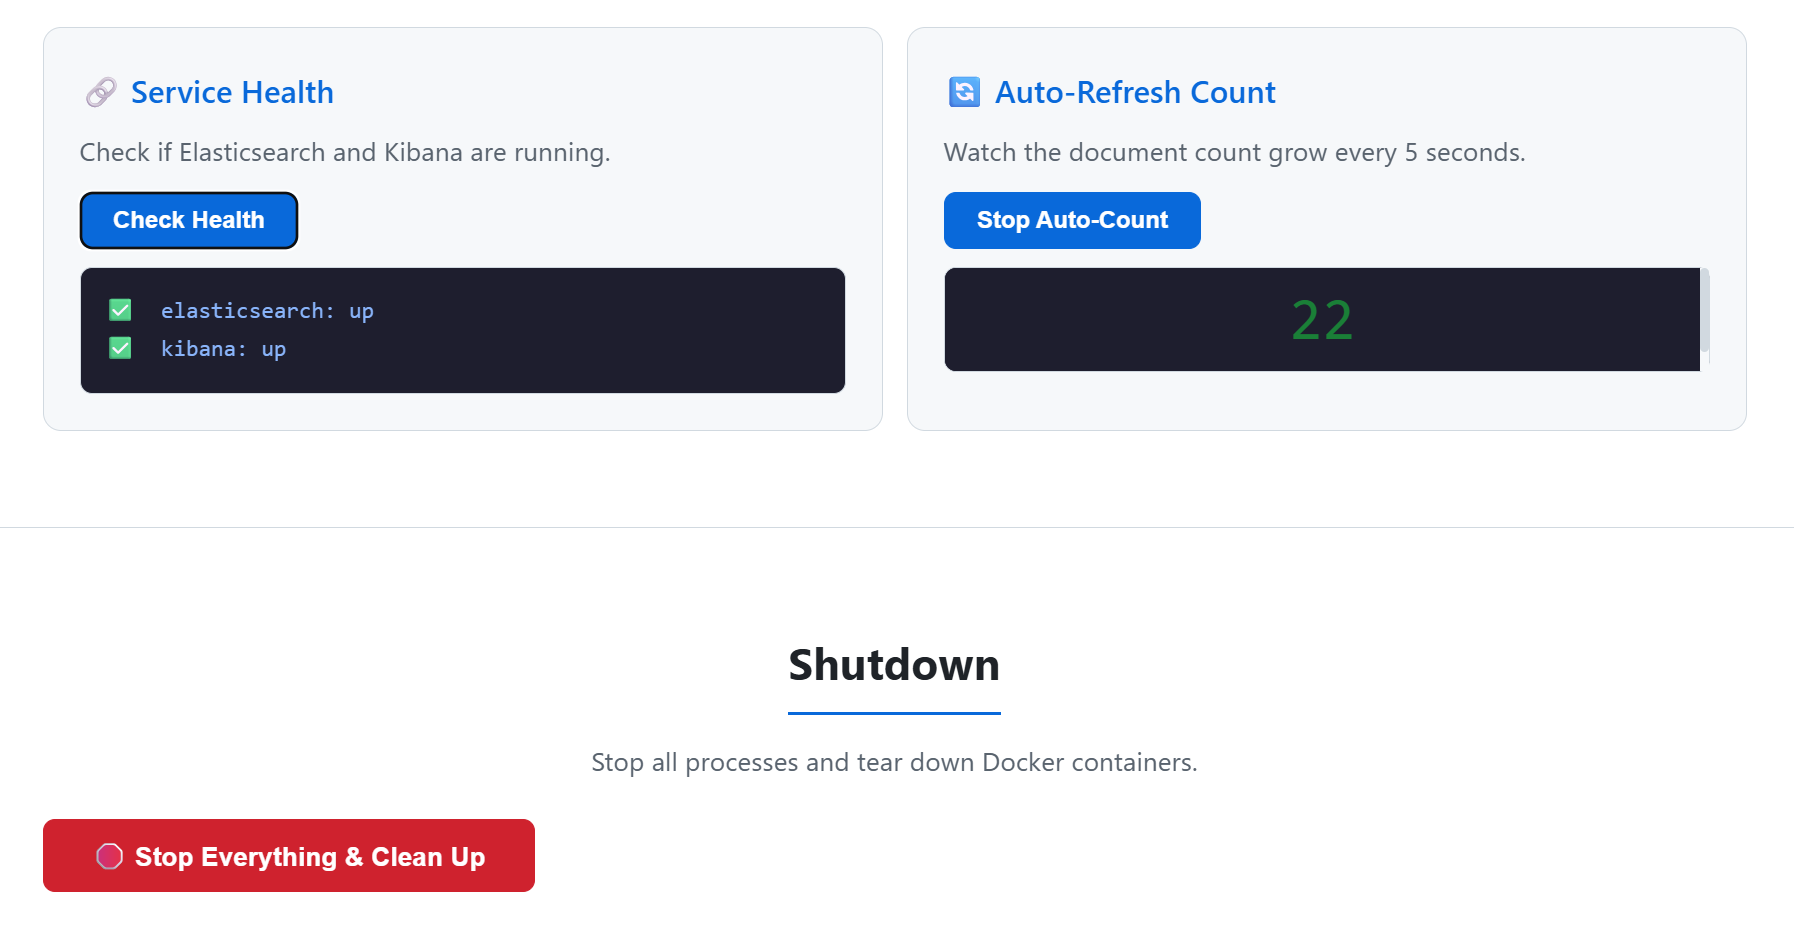
\includegraphics[width=\textwidth]{fig14_elasticsearch_docs.png}
    \caption{Index Elasticsearch \texttt{streamsight-trades} affichant les documents stock\'es. Chaque document correspond \`a une fen\^etre d'agr\'egation de 10 secondes et contient l'ensemble des m\'etriques calcul\'ees, y compris le VWAP, le Z-score et la classification d'anomalie.}
    \label{fig:elasticsearch_docs}
\end{figure}

%----------------------------------------------------------------------------------------
%	7. TOL\'ERANCE AUX PANNES ET FIABILIT\'E
%----------------------------------------------------------------------------------------
\section{Tol\'erance aux pannes et fiabilit\'e}

\subsection{Points de contr\^ole (Checkpointing)}
Spark Structured Streaming est configur\'e pour utiliser un r\'epertoire de points de contr\^ole. \`A chaque intervalle de d\'eclenchement, Spark sauvegarde les offsets Kafka courants et l'\'etat d'agr\'egation (sommes interm\'ediaires pour le VWAP) sur le disque. En cas de panne, l'application peut red\'emarrer et reprendre exactement l\`a o\`u elle s'est arr\^et\'ee, garantissant qu'aucune donn\'ee n'est perdue ni comptabilis\'ee en double.

\subsection{Watermarking}
Le watermark de 5 secondes est essentiel pour une agr\'egation correcte des fen\^etres. Il permet au syst\`eme d'attendre les donn\'ees arrivant en retard (\`a cause de la latence r\'eseau) avant de finaliser le r\'esultat de la fen\^etre. Les fen\^etres ne sont \'ecrites vers le sink qu'une fois que l'horloge de temps \'ev\'enementiel d\'epasse \texttt{window\_end + watermark}, garantissant la compl\'etude des r\'esultats.

\subsection{\'Ecritures idempotentes}
Pour atteindre une s\'emantique exactly-once de bout en bout, nous construisons un identifiant de document d\'eterministe pour Elasticsearch :

\begin{infobox}
\texttt{doc\_id = symbol + "\_" + window\_start\_timestamp}

\vspace{4pt}
\small Si une panne provoque le retraitement d'un batch par Spark, celui-ci g\'en\`ere exactement le m\^eme identifiant de document. Elasticsearch traite cela comme un \textbf{upsert} (mise \`a jour), garantissant que la m\^eme fen\^etre n'est jamais dupliqu\'ee dans la base de donn\'ees.
\end{infobox}

%----------------------------------------------------------------------------------------
%	8. LIMITATIONS ET TRAVAUX FUTURS
%----------------------------------------------------------------------------------------
\section{Limitations et travaux futurs}

\begin{itemize}
    \item \textbf{Robustesse statistique :} Le Z-Score actuel est calcul\'e en utilisant des statistiques d\'eriv\'ees de la \textit{m\^eme} fen\^etre. Une approche plus robuste consisterait \`a utiliser une comparaison par fen\^etre glissante (par exemple, comparer le VWAP actuel \`a la moyenne des 50 fen\^etres pr\'ec\'edentes).
    \item \textbf{Contrainte de symbole unique :} Le syst\`eme ne surveille actuellement que la paire BTC/USDT. La mise \`a l'\'echelle vers la surveillance de l'ensemble du march\'e n\'ecessiterait le partitionnement du topic Kafka par symbole et la mise \`a l'\'echelle des consommateurs Spark.
    \item \textbf{Mode de d\'eploiement :} Le prototype fonctionne en mode \texttt{local[*]}. Un d\'eploiement en production utiliserait un gestionnaire de cluster comme Kubernetes ou YARN pour distribuer la charge de travail sur plusieurs n\oe uds.
    \item \textbf{Syst\`eme d'alerte :} Actuellement, les anomalies sont stock\'ees de mani\`ere passive. Une it\'eration future devrait int\'egrer une couche d'alerte (par exemple, envoyer des notifications vers Slack ou PagerDuty) lorsqu'une anomalie est d\'etect\'ee.
    \item \textbf{R\'esilience WebSocket :} Le producteur n'impl\'emente pas de logique de reconnexion automatique. Un syst\`eme de production n\'ecessiterait une strat\'egie de r\'eessai avec backoff exponentiel lors d'une d\'econnexion.
\end{itemize}

%----------------------------------------------------------------------------------------
%	9. CONCLUSION
%----------------------------------------------------------------------------------------
\section{Conclusion}

STREAMSIGHT d\'emontre avec succ\`es l'impl\'ementation d'un pipeline moderne et \'evolutif d'ing\'enierie de donn\'ees en temps r\'eel. En int\'egrant Apache Kafka pour la mise en tampon, Spark Structured Streaming pour le traitement complexe avec \'etat, et Elasticsearch pour l'analytique, le syst\`eme atteint une latence inf\'erieure \`a la minute dans la d\'etection des anomalies du march\'e des cryptomonnaies.

Le projet met en lumi\`ere le passage des architectures batch aux architectures de streaming dans la technologie financi\`ere, illustrant comment des outils open source peuvent \^etre compos\'es pour r\'esoudre des probl\`emes complexes de donn\'ees \`a haute v\'elocit\'e. L'utilisation d'un watermarking strict et d'un stockage idempotent garantit l'int\'egrit\'e des donn\'ees, rendant l'architecture adapt\'ee \`a un d\'eveloppement ult\'erieur en un outil de support au trading de qualit\'e production.

%----------------------------------------------------------------------------------------
%	R\'EF\'ERENCES
%----------------------------------------------------------------------------------------
\section*{R\'ef\'erences}
\addcontentsline{toc}{section}{R\'ef\'erences}

\begin{thebibliography}{9}

\bibitem{kafka}
Apache Software Foundation.
\textit{Apache Kafka Documentation}.
Disponible : \url{https://kafka.apache.org/documentation/}

\bibitem{spark}
Apache Software Foundation.
\textit{Structured Streaming Programming Guide}.
Disponible : \url{https://spark.apache.org/docs/latest/structured-streaming-programming-guide.html}

\bibitem{elastic}
Elastic NV.
\textit{Elasticsearch Guide (8.11)}.
Disponible : \url{https://www.elastic.co/guide/en/elasticsearch/reference/current/index.html}

\bibitem{binance}
Binance.
\textit{Binance Spot API Docs}.
Disponible : \url{https://binance-docs.github.io/apidocs/spot/en/}

\bibitem{stats}
Freedman, D., Pisani, R., et Purves, R. (2007).
\textit{Statistics (4th ed.)}. W. W. Norton \& Company.

\end{thebibliography}

\end{document}
